\documentclass[11pt,a4paper]{article}

\usepackage[T1]{fontenc}
\usepackage[utf8]{inputenc}
\usepackage[polish]{babel}
\usepackage{graphicx}
\usepackage[a4paper,margin=2.5cm]{geometry}
\usepackage{microtype}

\title{Przykładowa analiza danych}
\author{Autor pracy magisterskiej}
\date{\today}

\begin{document}
\maketitle

\section{Cel analizy}

Celem tego krótkiego przykładu jest pokazanie prostego przepływu pracy w
programistycznej pracy magisterskiej. Dane źródłowe są przechowywane w pliku
CSV, skrypt napisany w języku Python przetwarza je i zapisuje wykres, a dokument
LaTeX wykorzystuje gotowy obraz. Dzięki temu obliczenia i tekst pozostają
rozdzielone, ale cały wynik można odtworzyć na innym komputerze.

\section{Wyniki}

Przykładowy zbiór opisuje liczbę użytkowników w kolejnych miesiącach. Na
rysunku~\ref{fig:wzrost} widoczny jest systematyczny wzrost analizowanej
wartości. W prawdziwej pracy ten sam schemat może służyć do prezentowania
wyników eksperymentów, symulacji numerycznych albo estymacji modelu.

\begin{figure}[ht]
    \centering
    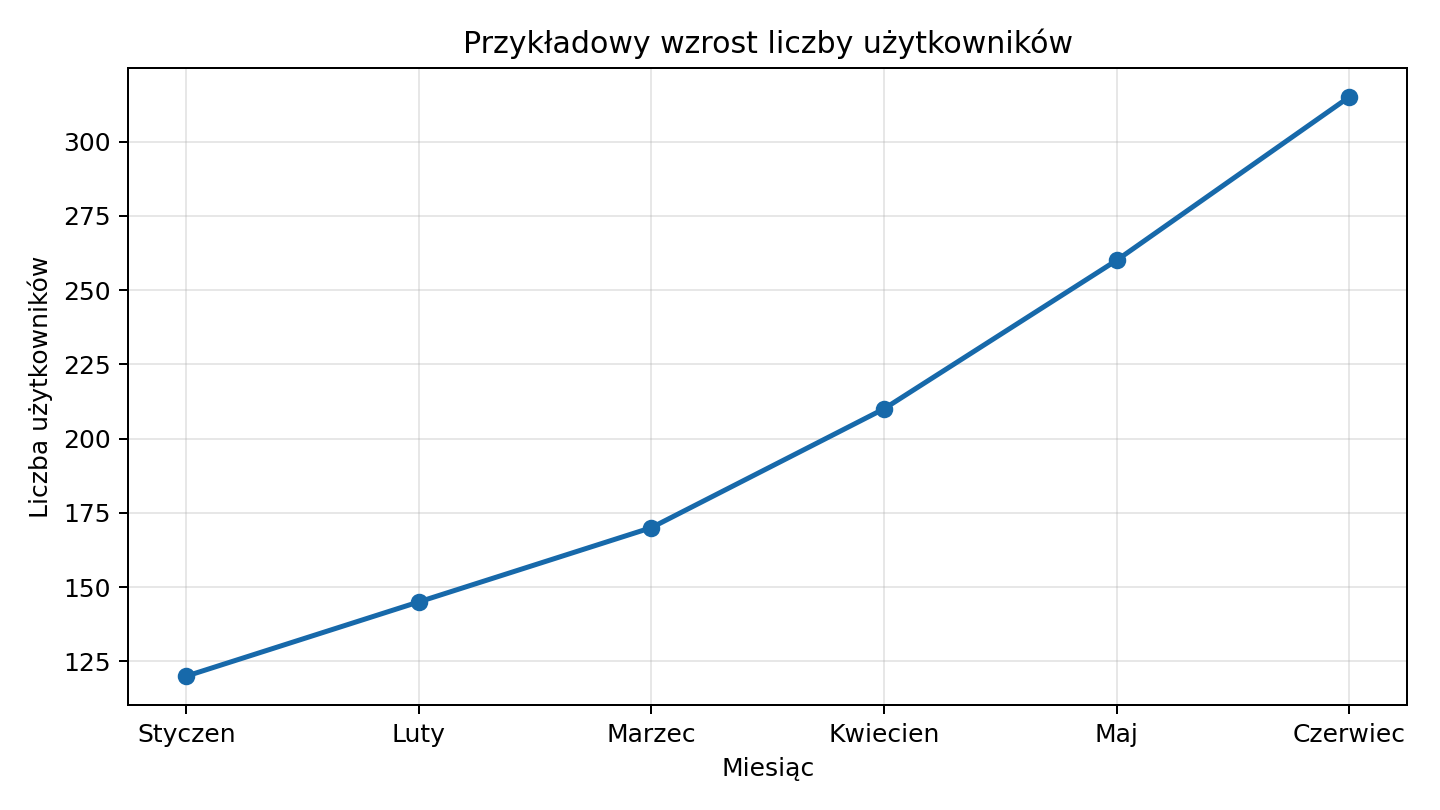
\includegraphics[width=0.82\textwidth]{obrazy/wykres.png}
    \caption{Liczba użytkowników w kolejnych miesiącach.}
    \label{fig:wzrost}
\end{figure}

Kod, dane i dokument powinny być przechowywane w repozytorium Git. Pozwala to
śledzić historię zmian, wracać do wcześniejszych wersji i bezpiecznie
publikować kolejne etapy pracy w serwisie GitHub.

\end{document}
